\documentclass[12pt,oneside,a4paper]{article}

%------------------------------------------------------------------------
%                         PACOTES UTILIZADOS
%------------------------------------------------------------------------
\usepackage{amssymb,amsmath,amsfonts,pgf,verbatim, graphicx,epsf,xcolor,color,tikz,hyperref}
\usepackage[brazilian]{babel}
\usepackage[utf8]{inputenc}
\usepackage[T1]{fontenc}
\usepackage{indentfirst}
\usepackage{lmodern}
%\usepackage{figure}
%--------------------------------------------------------------------------

%--------------------------------------------------------------------------
%                             MARGENS
%--------------------------------------------------------------------------
\usepackage{geometry}
\geometry{lmargin=3.0cm,rmargin=2.0cm,tmargin=3.0cm,bmargin=2cm}
%\setlength{\textwidth}{160mm}  %-------- largura do texto --------------
%\setlength{\textheight}{247mm} %------- altura do texto ---------------
%\setlength{\voffset}{-42mm} 
%\setlength{\hoffset}{-9mm}
%--------------------------------------------------------------------------

%--------------------------------------------------------------------------
%                             ESPAÇAMENTO ENTRE LINHAS
%--------------------------------------------------------------------------
\renewcommand{\baselinestretch}{1.0}
\parskip 7pt
%--------------------------------------------------------------------------

%--------------------------------------------------------------------------
%                              AMBIENTES E NUMERAÇÃO
%--------------------------------------------------------------------------
\newtheorem{Teorema}{Teorema}[section]
\newtheorem{Lema}{Lema}[section]
\newtheorem{Corolario}{Corol\'ario}[section]
\newtheorem{Proposicao}{Proposição}[section]
\newtheorem{Definicao}{Defini\c{c}\~ao}[section]
\newtheorem{Observacao}{Observa\c{c}\~ao}[section]
%--------------------------------------------------------------------------

%--------------------------------------------------------------------------
%                             NORMAS ABNT
%--------------------------------------------------------------------------
%       https://www.bco.ufscar.br/servicos-informacoes/normalizacao
%--------------------------------------------------------------------------


%--------------------------------------------------------------------------
%                            Legenda de figuras e tabelas
%--------------------------------------------------------------------------
\usepackage[figurename=Fig.,tablename=Tab.,footnotesize,bf]{caption}
%--------------------------------------------------------------------------


%--------------------------------------------------------------------------
%  INÍCIO DO DOCUMENTO. NÃO ALTERAR O PREÂMBULO, EXCETO TÍTULO E AUTORES.  
%--------------------------------------------------------------------------
\begin{document}
\pretolerance10000 %it does not allow separation syllabic.
%--------------------------------------------------------------------------


%--------------------------------------------------------------------------
%                             ESTILO DA PÁGINA (NÃO ALTERAR)
%--------------------------------------------------------------------------
\thispagestyle{empty}


%-------------------------------------------------------
% COM LOGO DA UFSCAR E DA BIENAL (requer as imagens)
%-------------------------------------------------------

\begin{minipage}{2.7cm}

\includegraphics[width=1.5\textwidth]{UFRN2.png}
\end{minipage}
\hfill 
% PARA INCLUIR O LOGO DE SUA INSTITUIÇÃO BASTA SALVAR O LOGO COM O NOME Logo_instituicao.png NA PASTA FIGURAS. CASO PREFIRA DEIXAR SEM O LOGO SUBSTITUA ABAIXO O NOME Logo_Instituicao.png POR Sem_Logomarca.png 
\begin{minipage}{2.7cm}
%\includegraphics[width=1\textwidth]{Figuras/Logo_instituicao.png}
\end{minipage}
\begin{minipage}{2.7cm}
    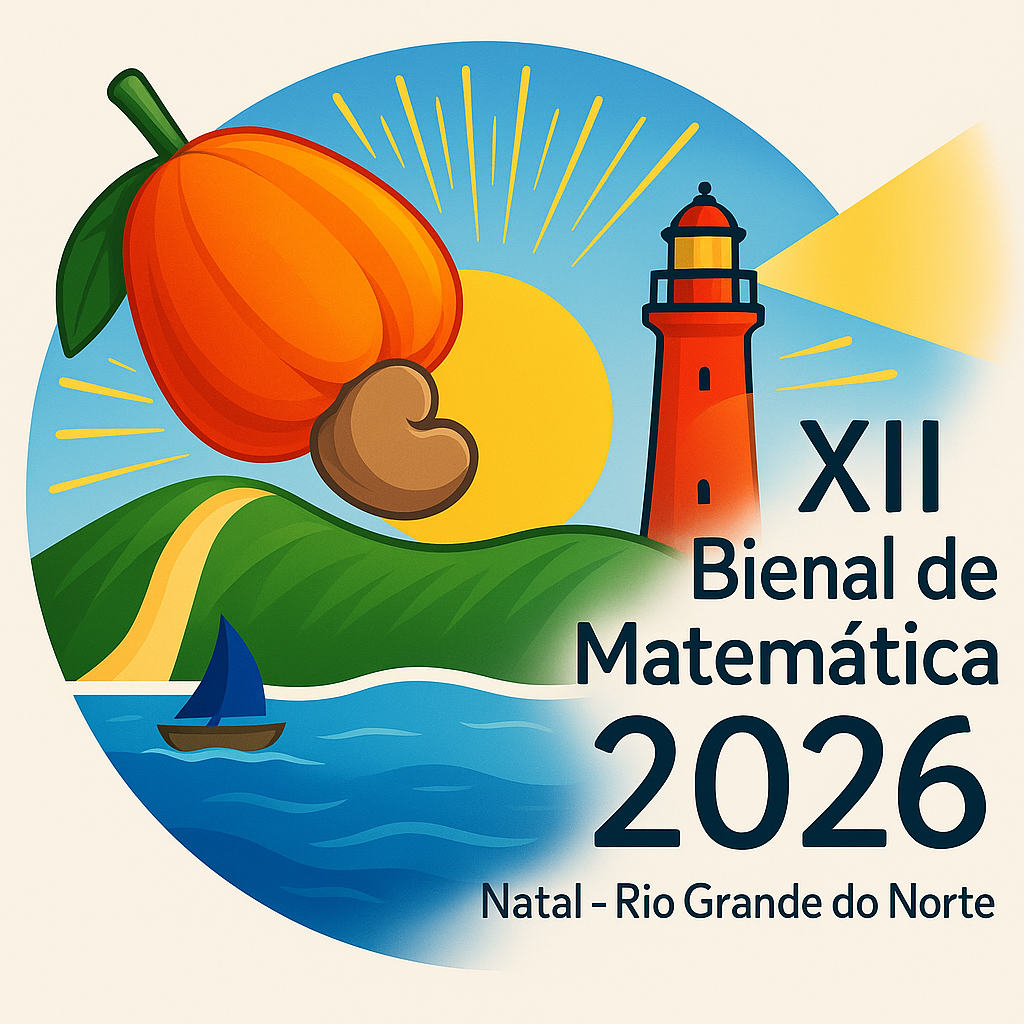
\includegraphics[width=1.2\textwidth]{LogoXIIBienal.png}
\end{minipage}




\pagenumbering{arabic}
\pagestyle{myheadings}
\markboth{XII BIENAL DE MATEM\'ATICA\, \textcolor[RGB]{245,159,50}{\bf 2024}}{XII BIENAL DE MATEM\'ATICA\, \textcolor[RGB]{245,159,50}{\bf 2026}}
%\markright{XI BIENAL DE MATEMÁTICA.\\ UNIVERSIDADE FEDERAL DE SÃO CARLOS.}


%--------------------------------------------------------------------------



%--------------------------------------------------------------------------
%                   IDENTIFICAÇÃO DO TRABALHO E DOS AUTORES
%--------------------------------------------------------------------------
\vspace{1.0cm}

\begin{center}
	{\LARGE \bf
		
		MINICURSO%\footnote{Este trabalho foi apoiado ...}
		
}\end{center}


\begin{center}
{\Huge\bf

       T\'itulo de trabalho%\footnote{Este trabalho foi apoiado ...}

}\end{center}

\begin{center}
	{\large\bf
		
		Subt\'itulo de trabalho%(Se houver)
		
}\end{center}
%Use o comando \footnote{Este trabalho foi apoiado ...} logo após o título caso necessário indicar o apoio de agência/instituição.

\begin{center}
{\large

 Sobrenome 1, Nome 1\footnote{Afilia\c{c}\~ao. Este autor foi apoiado ...};
 Sobrenome 2, Nome 2\footnote{Afilia\c{c}\~ao. Este autor foi apoiado ...} e
 Sobrenome 3, Nome 3\footnote{Afilia\c{c}\~ao. Este autor foi apoiado ...}

}\end{center}
 %Use o comando \footnote{Afiliação. Este autor foi apoiado ...} logo após o nome do autor para identificar a Instituição do autor e caso necessário indicar o apoio de agência/instituição.


\noindent \textit{\textbf{Resumo:}}{\it 
  Este documento \'e um modelo para a formata\c{c}\~ao dos textos de trabalhos, minicursos e oficinas submetidos \'a XII BIENAL DE MATEM\'ATICA, que ocorrer\'a na Universidade Federal do  Rio Grande do Norte - Natal/RN, de 03 a 07 de agosto de 2026. 

O resumo deve ter, no m\'aximo, 250 palavras. (N\~ao alterar o estilo e tamanho das fontes deste documento.)
}

\begin{flushleft}
\textit{\textbf{Palavras-chave:}}{\it
palavra 1, palavra 2, palavra 3...  at\'e 5 palavras chaves.

}\end{flushleft}
%--------------------------------------------------------------------------

 

%--------------------------------------------------------------------------
%                             CONTEÚDO DO TRABALHO
%--------------------------------------------------------------------------


\section{\sc introdu\c{c}\~ao}


O arquivo deve ser enviado com o nome: \vspace{0.3cm}\\ XII\textunderscore BM\textunderscore MINICURSO\textunderscore eixo temático\textunderscore nome do autor\textunderscore último sobrenome.tex\\ 
exemplo:\vspace{0.3cm}\\
XII \textunderscore BM\textunderscore  MINICURSO\textunderscore T2\textunderscore Maria\textunderscore Silva.pdf.

Os textos devem ser formatados de acordo com estas instruções e este arquivo texto pode ser usado como um template. Estes estão limitados com no mínimo 1 e  no máximo 3 páginas, incluindo tabelas e figuras. O arquivo final em formato PDF não deve exceder 5 MB. Recomenda-se usar este arquivo para submeter o texto.

O texto deve ser digitado em papel tamanho A4, usando fonte Times New Roman, tamanho 10, exceto para o título e espaço simples entre linhas.

\subsection{Títulos e Subtítulos das Seções}

Os títulos e subtítulos das seções devem ser digitados em fonte Times New Roman, tamanho 12, estilo negrito, e alinhados à esquerda. Os títulos ser escritos em letras maiúsculas, enquanto nos subtítulos só as primeiras letras de cada palavra serão maiúsculas. Eles devem ser numera-dos, usando numerais arábicos separados por pontos. Uma linha em branco de espaçamento simples deve ser incluída acima e abaixo de cada título ou subtítulo

\textbf{Corpo do Texto}

O corpo do texto é justificado, com espaçamento simples. A primeira linha de cada parágrafo tem recuo de 0,6 cm a partir da margem esquerda.

As tabelas devem ser centralizadas. A legenda deve ser centralizada e localizada imediatamente acima da tabela. Uma linha em branco, em espaço simples, deve ser introduzida entre a tabela, seu título e o texto.

\begin{table}
	\centering
\begin{tabular}{c|c|c}
cabe\c calho 1&cabe\c calho 2&cabe\c alho 3\\
\hline
a&b&c\\
d&e&f\\
h&i&k
\end{tabular}
\caption{Autoria pr\'opria}
\end{table}

As figuras devem ser centralizadas. Sua legenda deve ser centralizada e localizada imediatamente acima da figura. Deve ser deixada uma linha em branco, de espaçamento simples, entre as figuras e o texto.

\begin{figure}[h!]
	\centering
	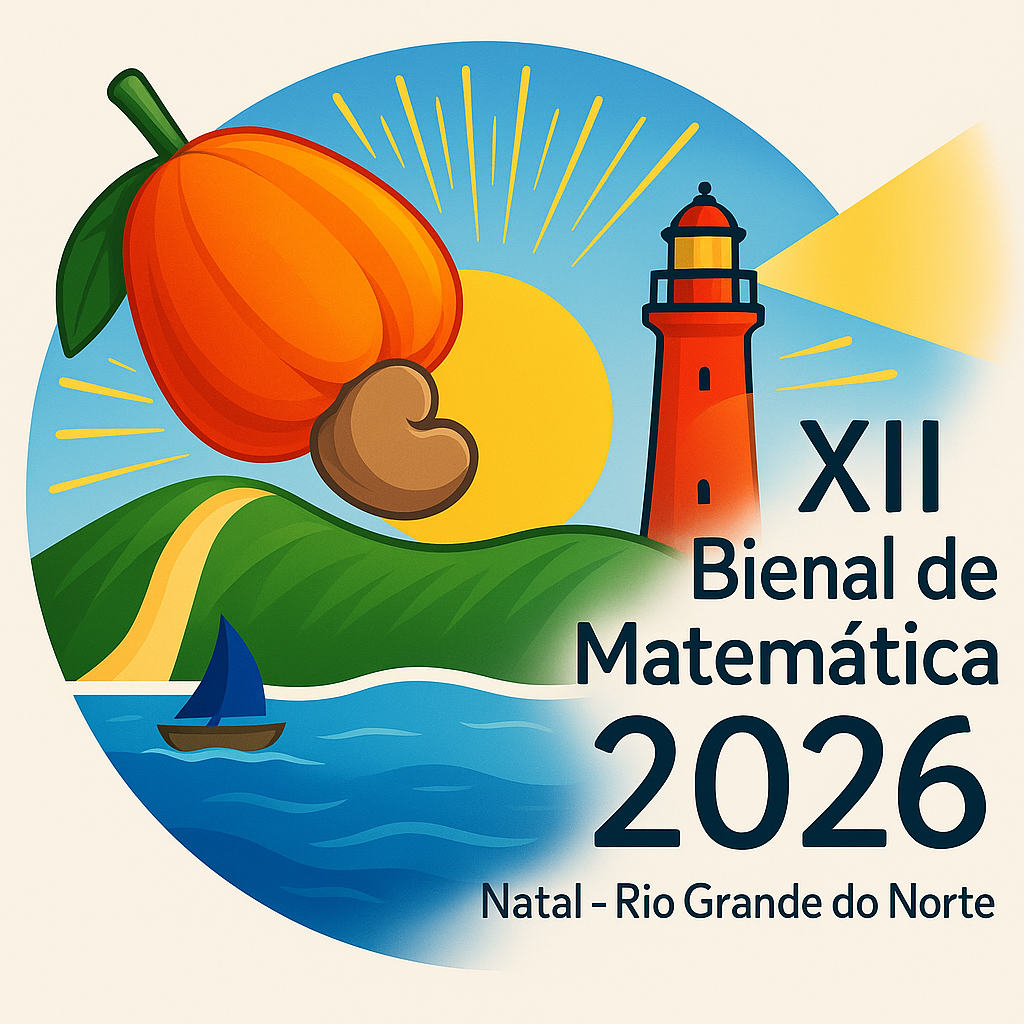
\includegraphics[width=7cm]{LogoXIIBienal.png}
   \caption{Autoria pr\'opria}
\end{figure}


\section{\sc conclus\~oes} %(SE HOUVER) 

As indicações de formatação de texto devem ser suprimidas na versão final do artigo antes do envio.


\renewcommand{\refname}{Bibliografia}
\addcontentsline{toc}{section}{Refer\^encias bibliogr\'aficas}
  \begin{thebibliography}{9}

%--------------------------------------------------------------------------
%                             NORMAS ABNT
%--------------------------------------------------------------------------
%       https://www.bco.ufscar.br/servicos-informacoes/normalizacao
%--------------------------------------------------------------------------

\bibitem{BURGER} BURGER, M.; HACKL, B.; RING, W. Incorporating topological derivatives into level set methods. \textbf{Journal of Computational Physics}, v. 194, n. 1, p. 344-362, 2004.

  
\bibitem{LITTLE} LITTLE, R. W. \textbf{Elasticity}. New Jersey: Prentice-Hall, 1973.


 
\end{thebibliography}



\end{document}

